\begin{frame}{}

\section{Voigt profile fitting}

\vspace*{1cm}

{\huge{\textbf{Voigt profile fitting}}}

\end{frame}



\begin{frame}{\textbf{Absorption species}}

\begin{figure}[!htbp]
  \centering
  \vspace{3mm}
  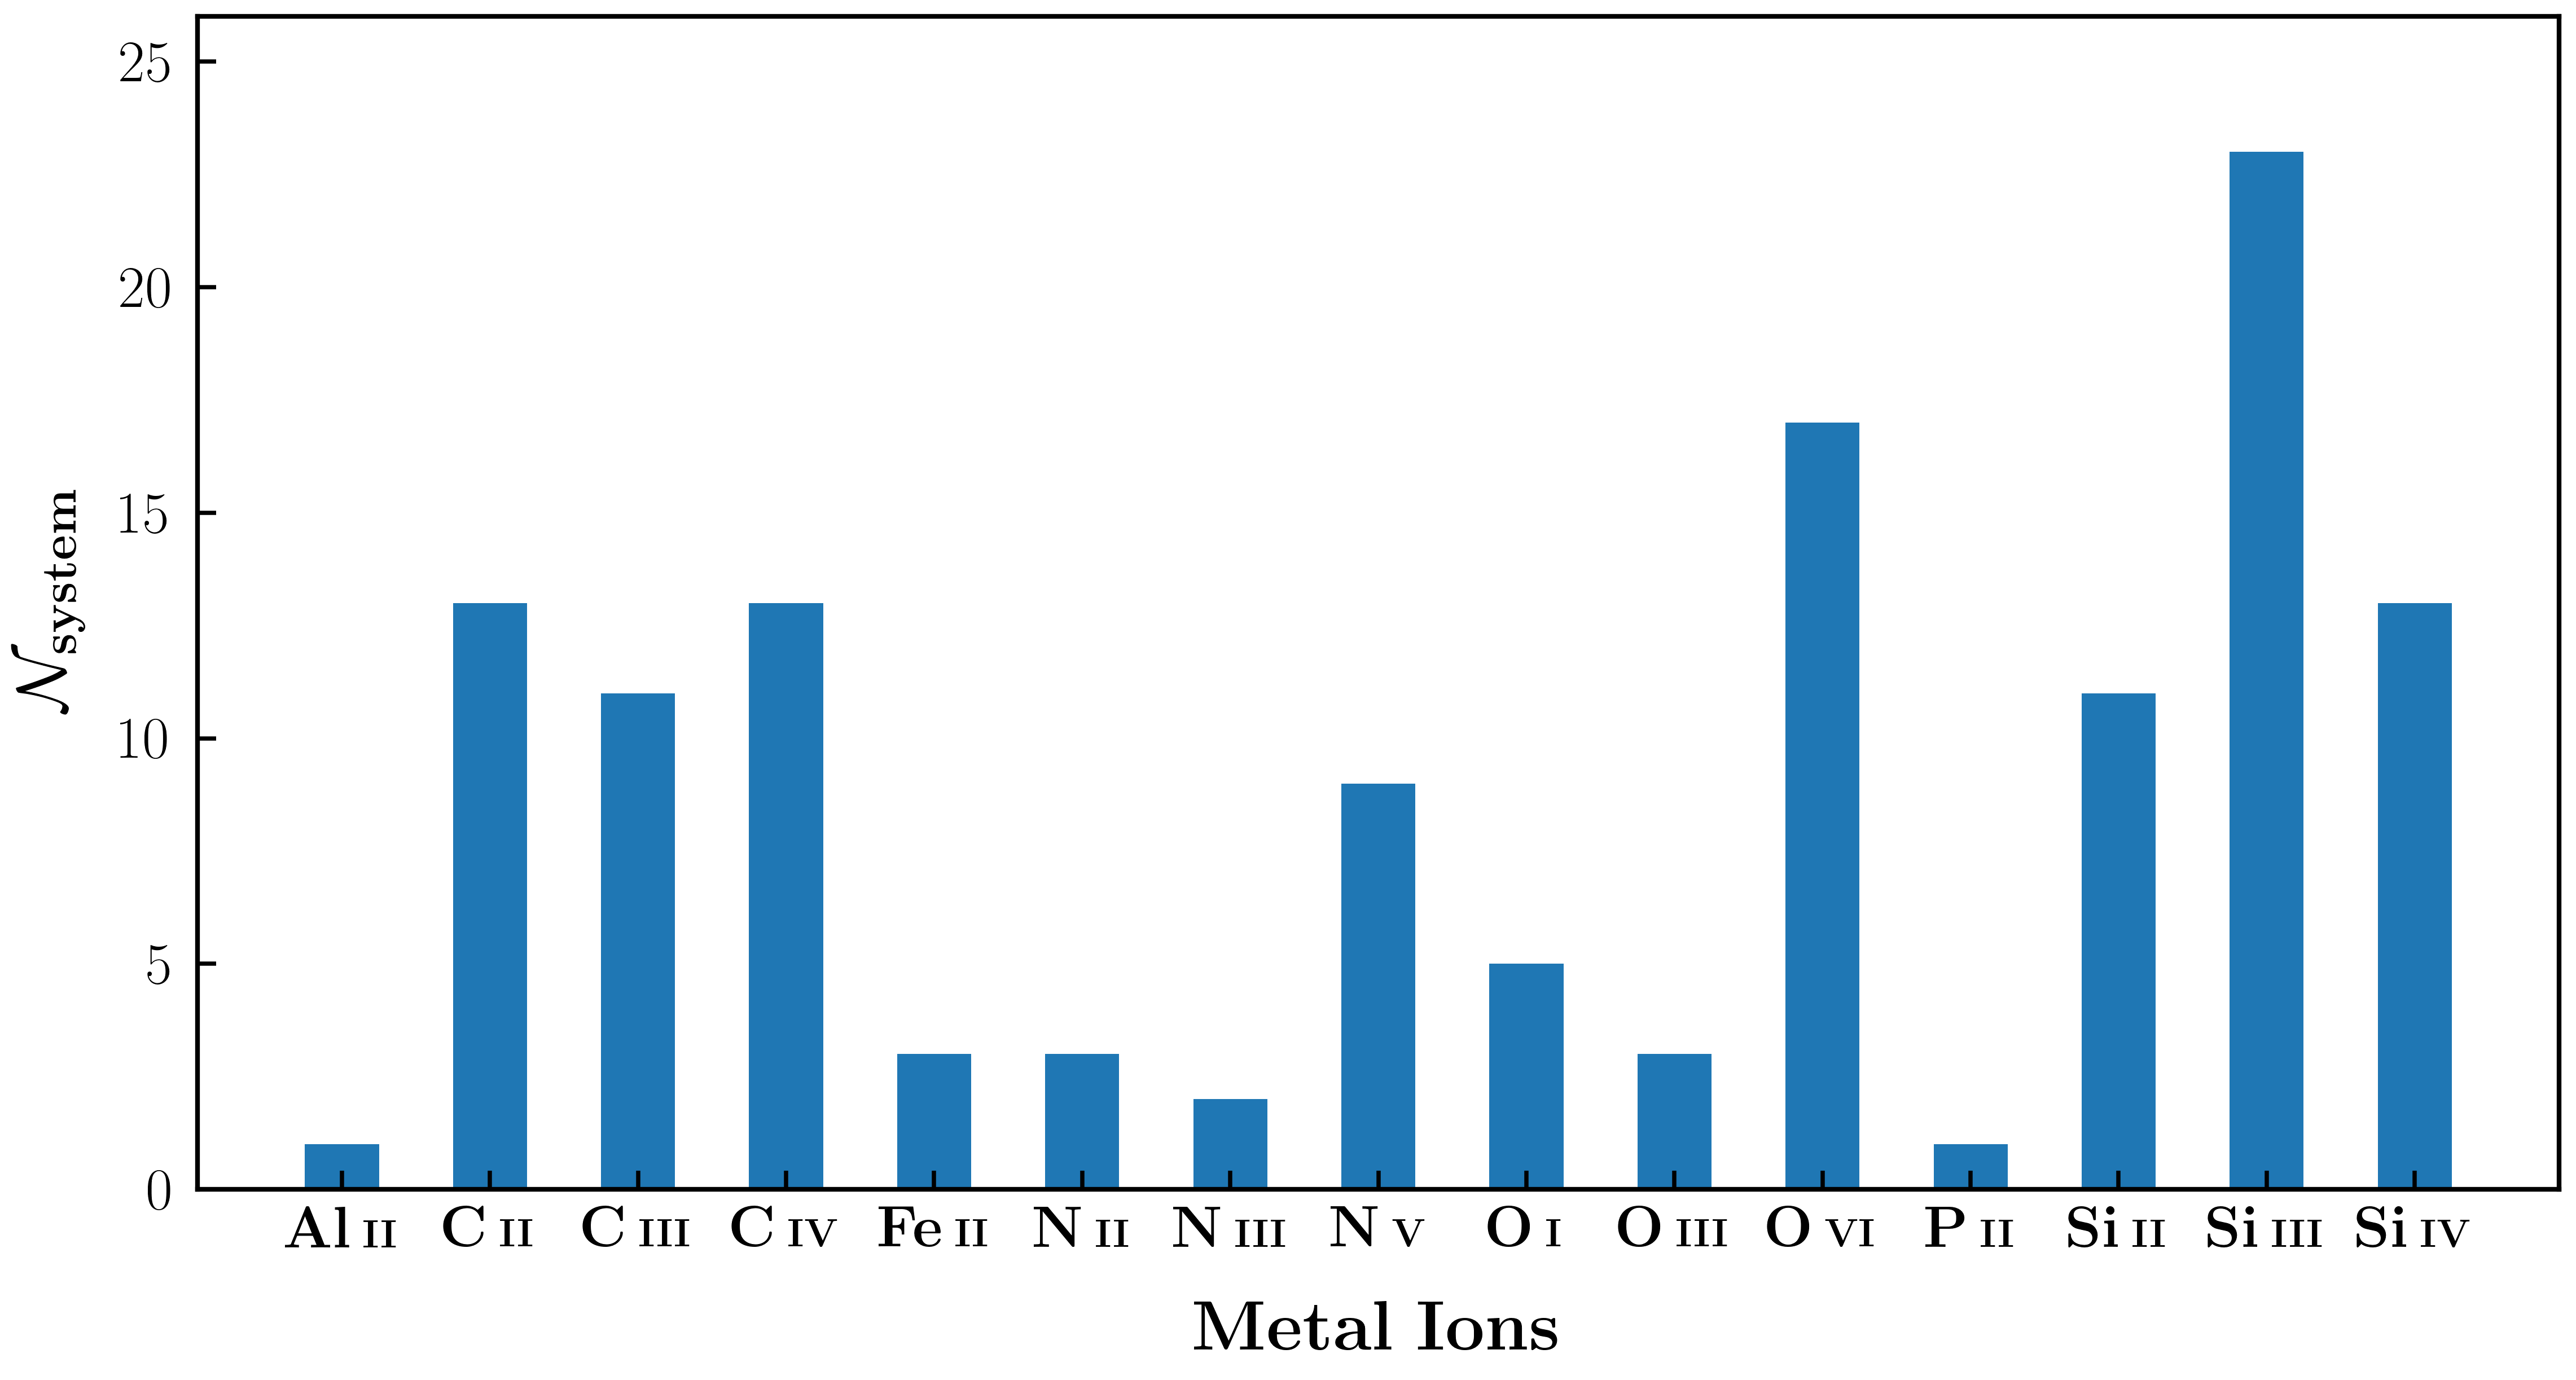
\includegraphics[width=11cm]{Figures-Thesis/metal-ion-system.png}
  \vspace*{-1mm}
  \caption{Distribution of metal species in 29 BLA candidates}
\end{figure}

\end{frame}


\begin{frame}[noframenumbering]{\textbf{Absorption species}}

  \begin{figure}[!htbp]
    \centering
    \vspace{3mm}
    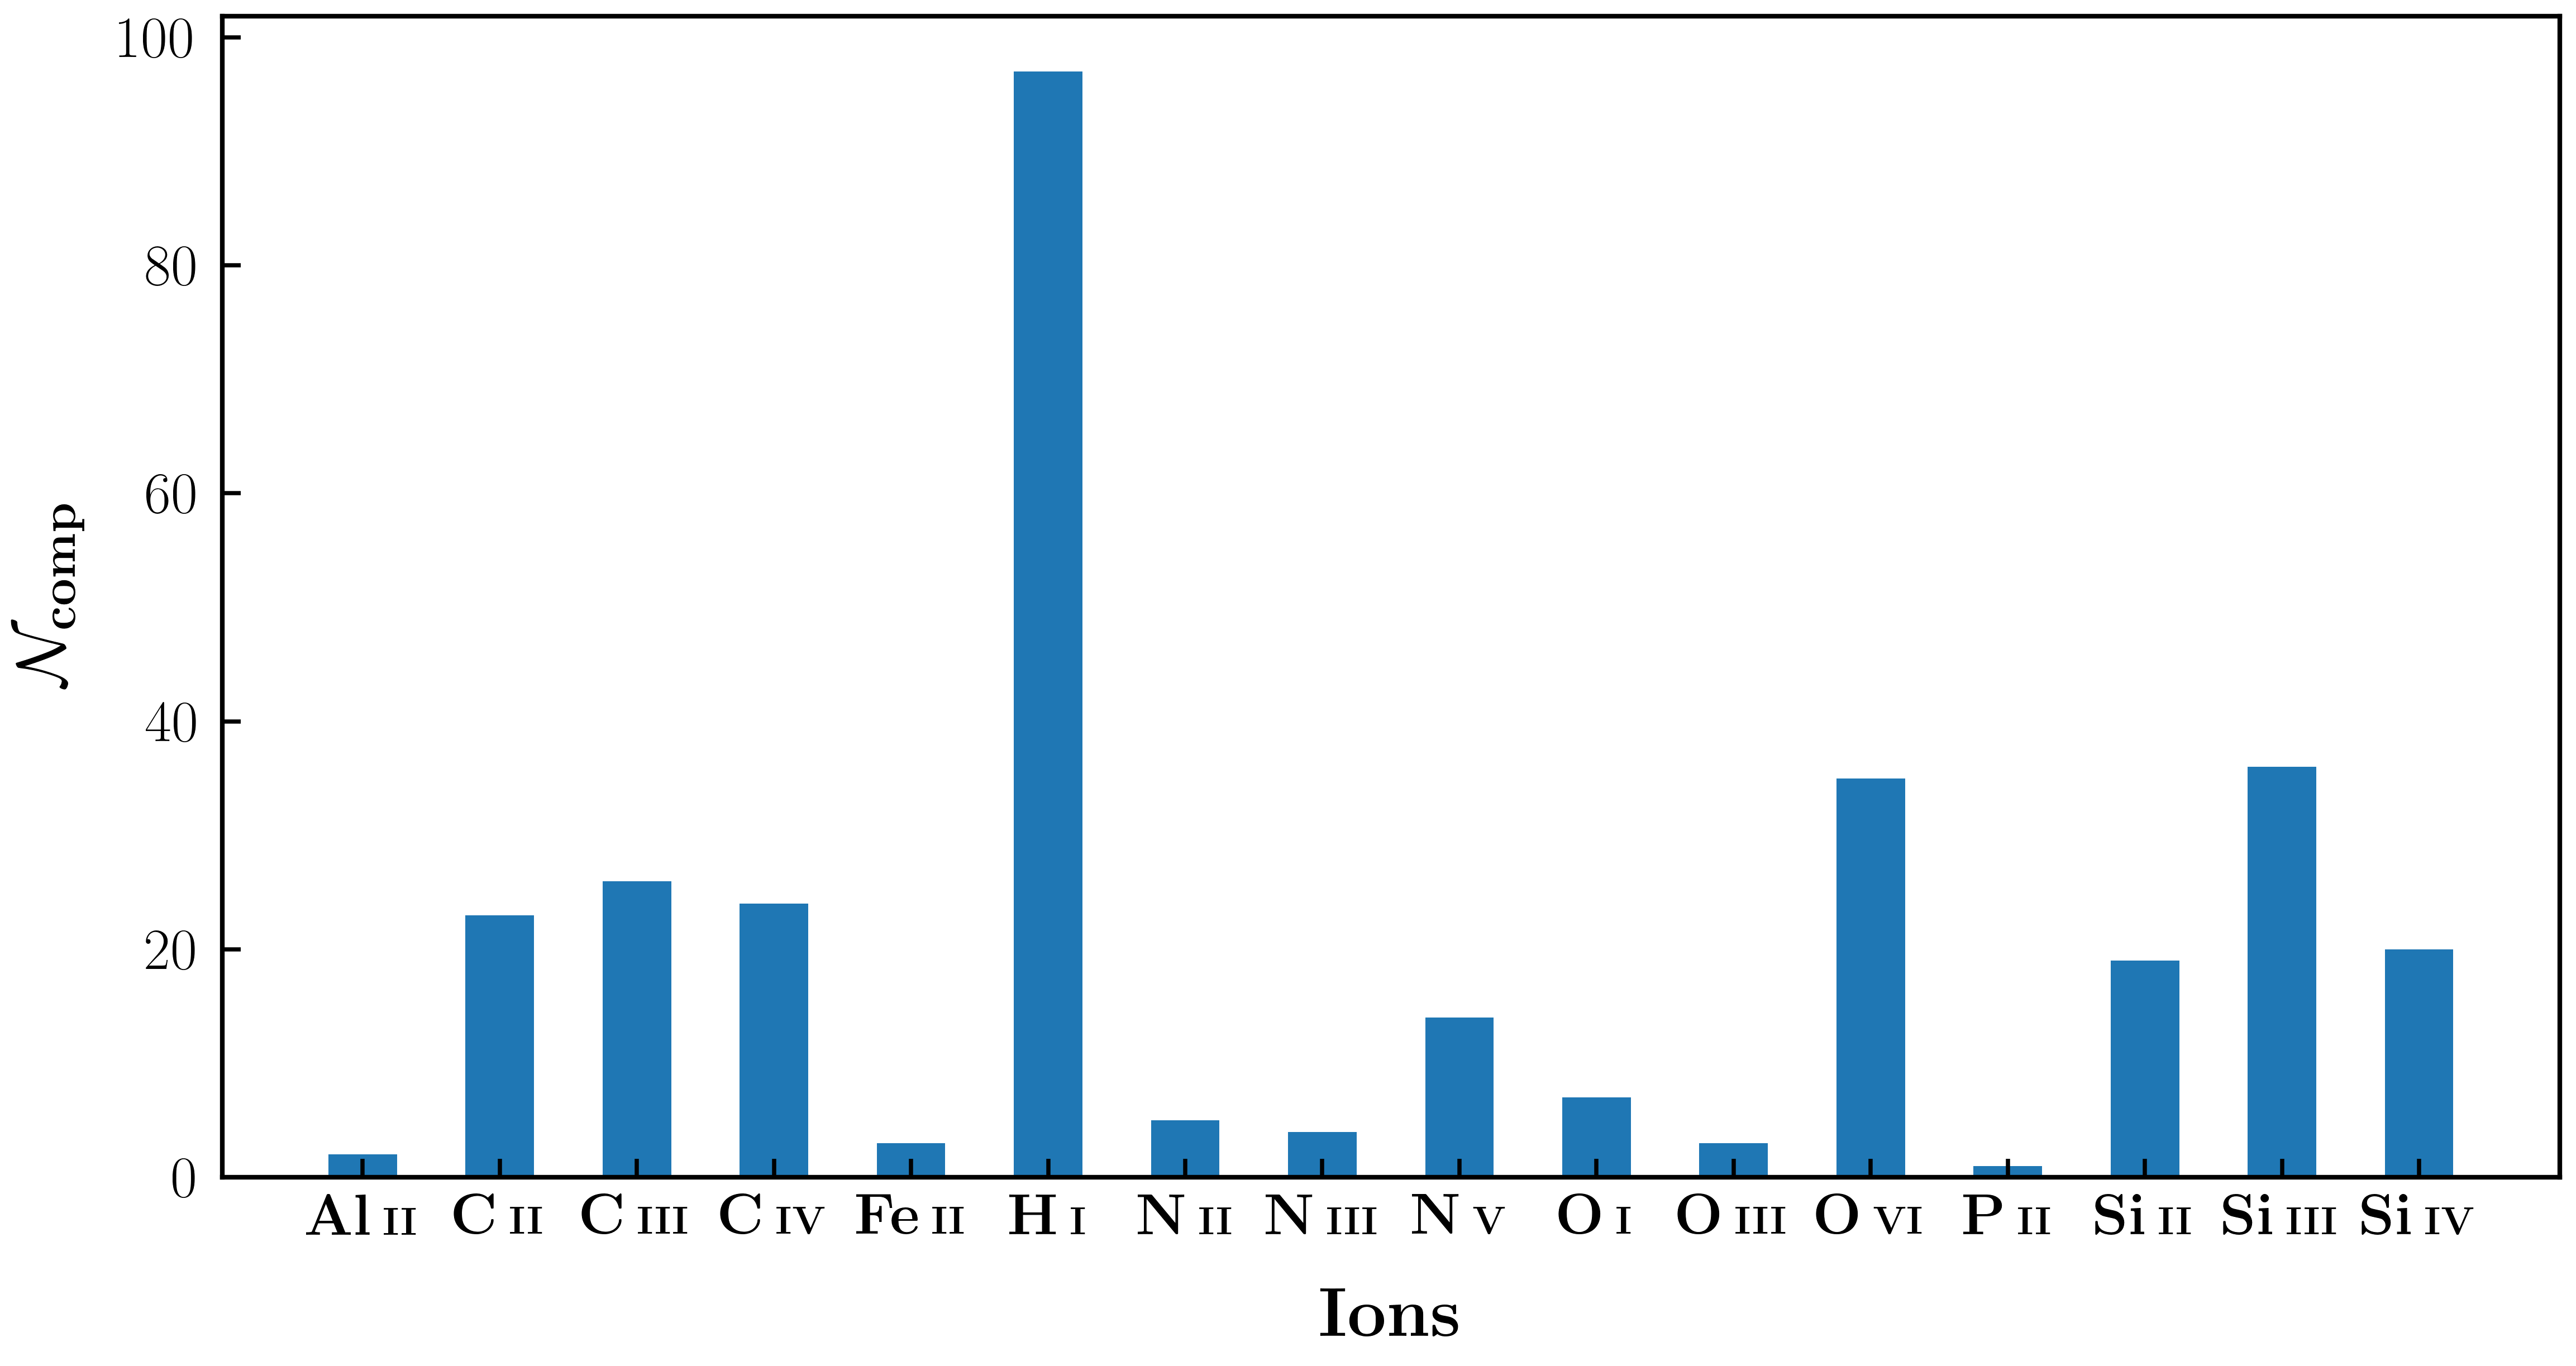
\includegraphics[width=11cm]{Figures-Thesis/ion-component.png}
    \vspace*{-1mm}
    \caption{Distribution of components of absorption species in 29 BLA candidates}
  \end{figure}
  
  \end{frame}


\begin{frame}{\textbf{N(\ion{H}{i}) and \emph{b}(\ion{H}{i})}}


 \uncover<2>{ \begin{figure}[!htbp]
  \centering
  \includegraphics<2->[width=11cm]{Figures-Thesis/NHi-bHi-distribution.png}
  \vspace*{-1mm}
  \caption{Distribution of column densities and Doppler widths of 97 \ion{H}{i} components}
\end{figure}}


\end{frame}


\begin{frame}[noframenumbering]{\textbf{N(\ion{H}{i}) and \emph{b}(\ion{H}{i})}}

\begin{figure}[!htbp]
  \centering
  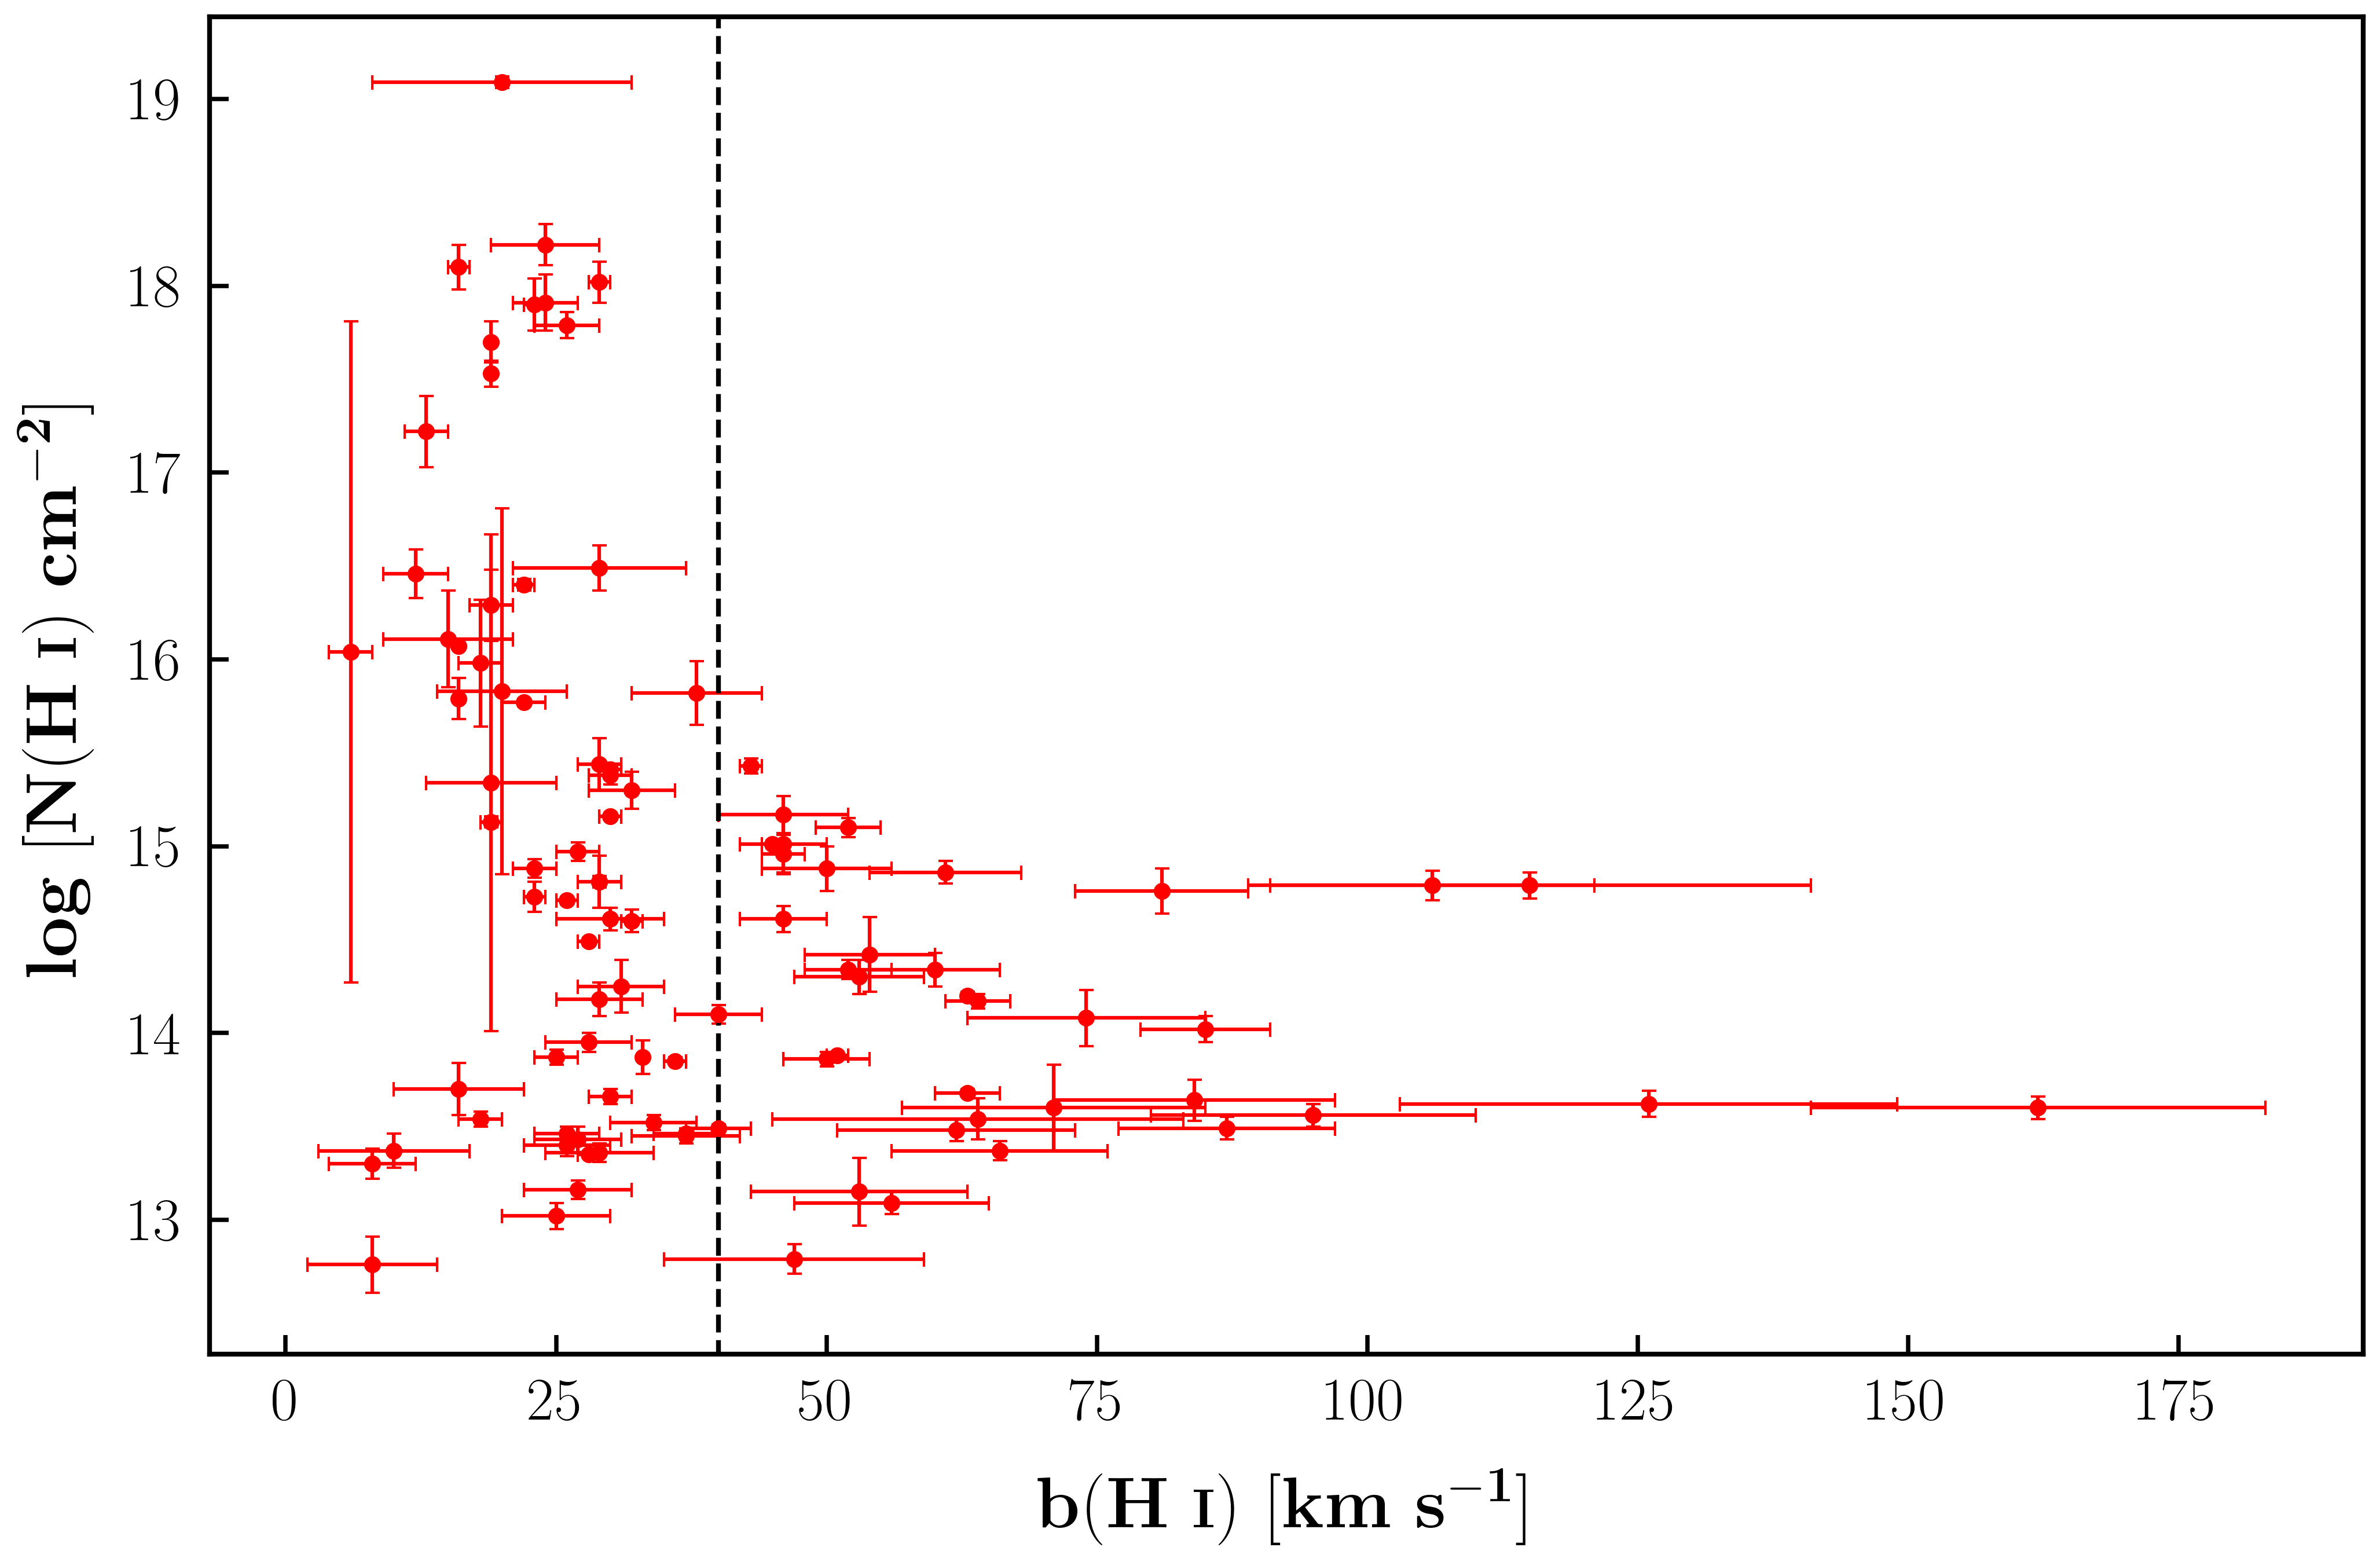
\includegraphics[width=9.5cm]{Figures-Thesis/NHi_vs_bHi.png}
  \vspace*{-1mm}
  \caption{\ion{H}{i} column density v/s Doppler width for 97 \ion{H}{i} components}
\end{figure}

\end{frame}


% \begin{frame}{\textbf{\emph{b}(\ion{O}{vi}) vs. \emph{b}(\ion{H}{i})}}

% \begin{columns}
%   \begin{column}{0.2\textwidth} 
%     \vspace*{-12mm}
%     \begin{figure}[!htbp]
%       \centering
%       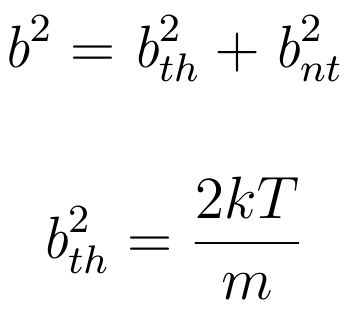
\includegraphics[width=2.5cm]{Figures/b.png}
%     \end{figure}
%     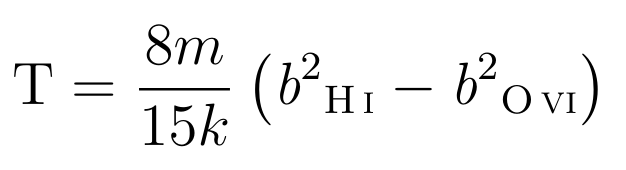
\includegraphics[width=4cm]{Figures/T.png}
    
%   \end{column}      

%   \begin{column}{0.8\textwidth}

%     \vspace*{-2mm}
%     \begin{figure}[!htbp]
%       \centering
%       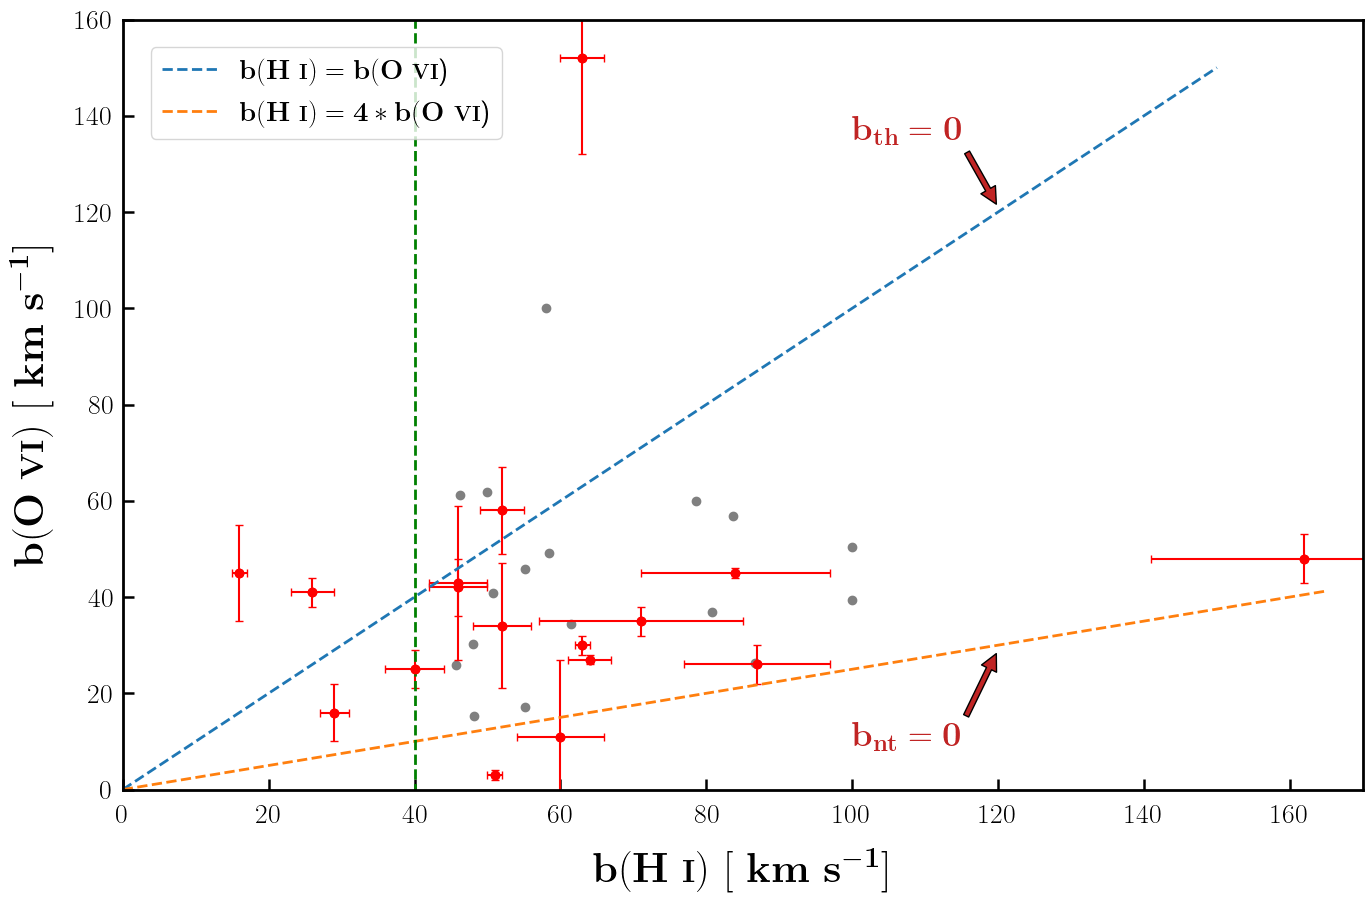
\includegraphics[width=9cm]{Figures/bHi_vs_BOvi_danforth.png}
%       \vspace*{-1mm}
%       \caption{\emph{b}(\ion{O}{vi}) vs. \emph{b}(\ion{H}{i}). Grey filled circles are measurements from Danforth et al. (2016).}
%     \end{figure}

%   \end{column}

% \end{columns}

% \end{frame}


% \begin{frame}[noframenumbering]{\huge{{\textbf{Insights}}}}


% \begin{columns}
%   \begin{column}{0.2\textwidth} 
%     \vspace*{-18mm}
%     \begin{figure}[!htbp]
%       \centering
%       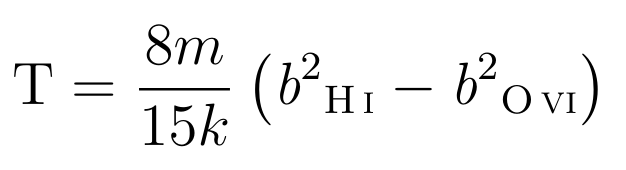
\includegraphics[width=3.5cm]{Figures/T.png}
%     \end{figure}
    
    
%   \end{column}      

%   \begin{column}{0.8\textwidth}

%     \vspace*{-5mm}

%     \begin{figure}[!htbp]
%       \centering
%       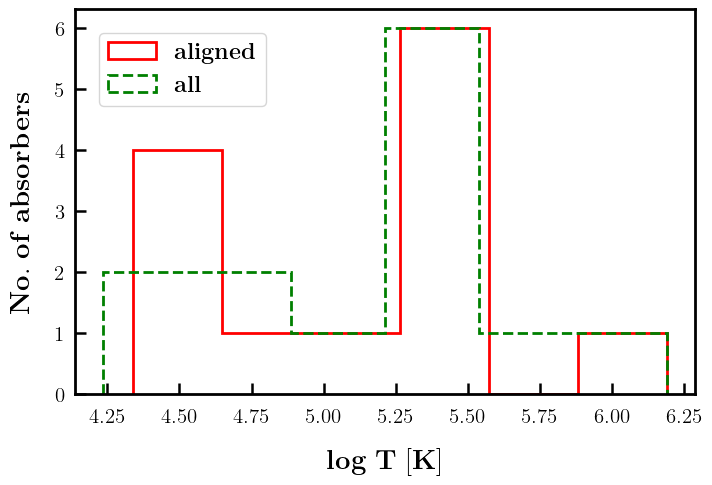
\includegraphics[width=9cm]{Figures/T_histogram.png}
%       \vspace*{-1mm}
%       \caption{Distribution of temperature calculated from Doppler parameters of \ion{H}{i} and \ion{O}{vi} lines.}
%     \end{figure}
%   \end{column}

% \end{columns}

% \end{frame}
